\section{Introduction}

The development of safe and reliable autonomous driving systems\citep{caesar2021nuplan, ding2023survey, hu2023planning, cui2024drive} has become a central focus in modern transportation research, aiming to enhance mobility, reduce accidents, and improve driving efficiency through advanced algorithmic design and large scale testing. Real world testing alone is infeasible as demonstrating human level safety statistically would require billions of kilometers and even such testing cannot exhaust the long tail of rare, safety critical ``edge cases". Simulation has therefore become an indispensable paradigm for autonomous driving validation. It enables scalable and efficient evaluation of driving algorithms, providing a repeatable and controllable environment to test rare, high risk interactions such as aggressive cut-ins or unpredictable pedestrians, which are essential for assessing real world robustness.

\begin{figure}[htbp]
    \centering
    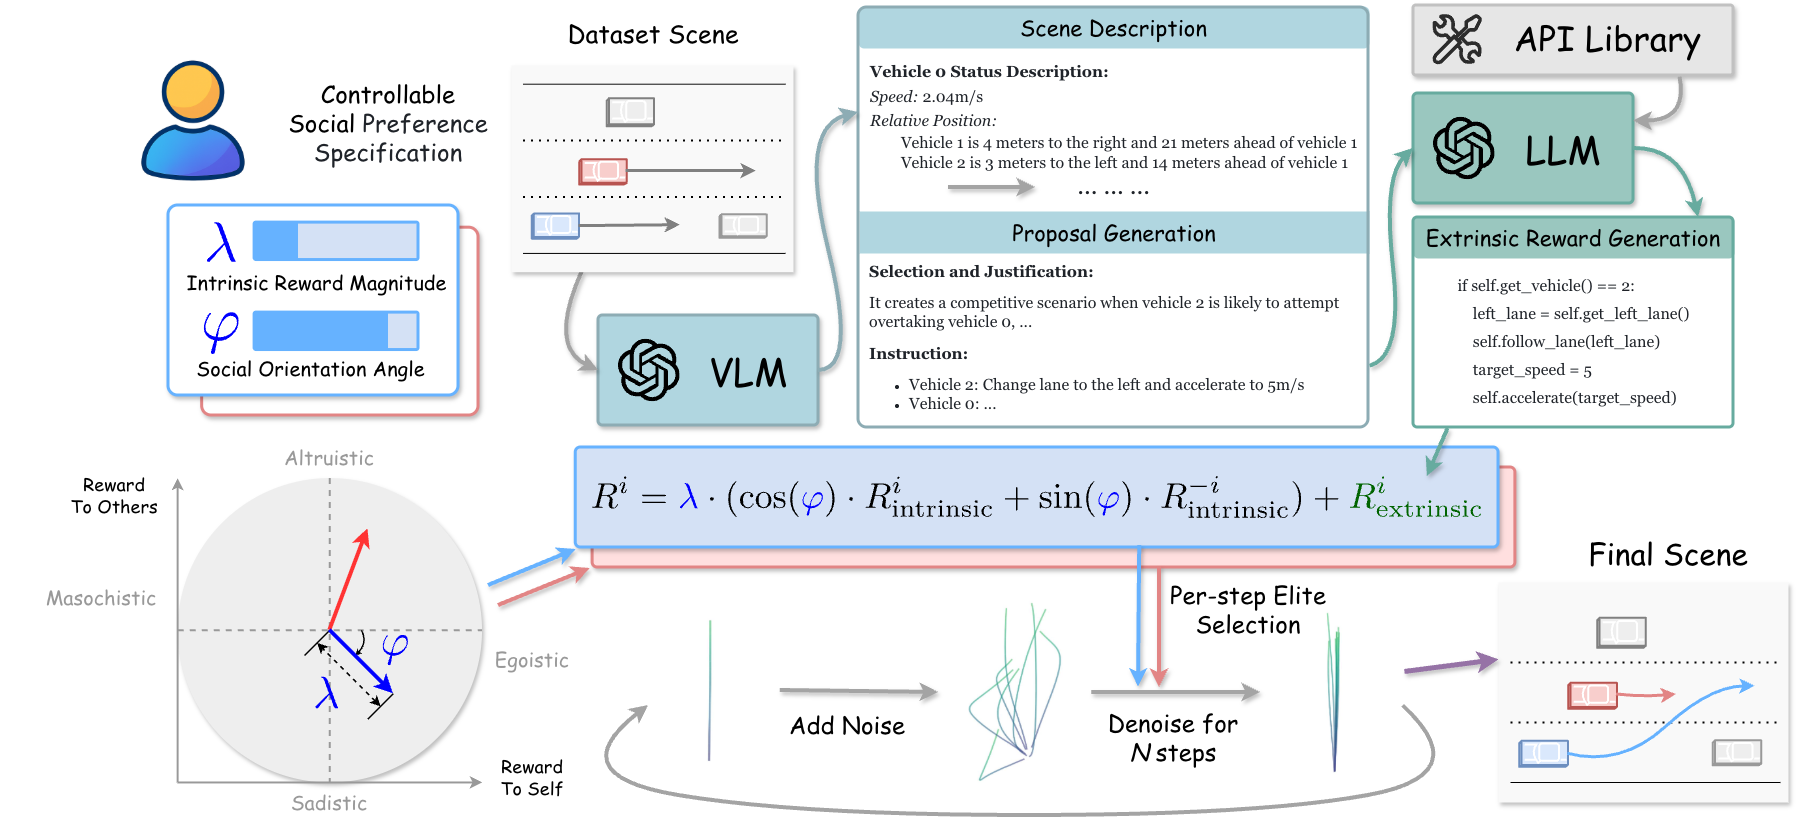
\includegraphics[width=1.0\textwidth]{figures/changan_new.drawio.png}
    \caption{Overview of \our. The framework leverages VLMs and LLMs to construct social rewards that guide a multi-agent diffusion process.}
    \vspace{-8pt}
    \label{fig:social-drive-gen}
\end{figure}

As simulation technology continues to evolve, the main focus of simulation fidelity has shifted from replicating only the physical world toward capturing the intricacies of human behavior and social interaction.  Early simulation research~\citep{feng2022trafficgen, ding2024realgen} emphasized accurate vehicle dynamics, sensor modeling, and photorealistic environments to ensure physical credibility. However, as autonomous driving systems increasingly engage in decision making and interaction with other agents, the need for behavioral and social realism has become crucial~\citep{zhan2019interaction}. Simulated social vehicles must display diverse strategies resembling human drivers, including cooperation, competition, negotiation, and occasional irrationality, to adequately assess the ability of modern driving policies~\citep{schwarting2019social, jin2024surrealdriver}. Traditional rule based traffic models~\citep{treiber2000congested} are computationally efficient but inherently limited in diversity, often producing overly deterministic and predictable behaviors~\citep{suo2021trafficsim}. 
% Game theoretic models provide a more principled framework for multi agent decision making but depend on assumptions of rationality that rarely hold in real traffic. 
Psychology inspired approaches using Social Value Orientation (SVO)~\citep{schwarting2019social} improve behavioral realism by modeling how agents balance self and others' rewards. While effective for predicting cooperative and competitive driving, current applications~\citep{dai2023socially} focus on limited and simplified scenarios. Extending SVO to dynamic, multi-agent contexts remains a key challenge for realistic social behavior modeling.

Recent progress in generative models provides new opportunities to address these challenges. Vision Language Models (VLMs) and Large Language Models (LLMs)~\citep{openai2023gpt4, liu2023visual} demonstrate strong reasoning and multimodal understanding, allowing them to serve as semantic planners that interpret driving scenes and propose high level interaction intents~\citep{xu2024drivegpt4, fu2024drive}. At the same time, diffusion models have become the leading approach for producing temporally coherent and physically consistent multi-agent trajectories. Integrating these paradigms by connecting high level intent reasoning from language models with trajectory generation from diffusion models has shown promising results~\citep{zhang2025drivegen}. However, current studies rarely incorporate social value modeling, which limits the diversity and social awareness of the generated interactions.

To overcome these limitations, we propose SocialDriveGen, a hierarchical framework that unites semantic reasoning, social psychology, and generative modeling to create controllable and socially realistic traffic scenarios. A VLM first analyzes scene context and proposes meaningful interactions between vehicles, which are then interpreted by an LLM into practical reward functions that define interpretable objectives for generation. Building upon this, a socially aware reward formulation explicitly represents egoism and altruism, offering fine grained control over driver personalities across the behavioral spectrum. Finally, a guided multi-agent diffusion model jointly synthesizes trajectories for all vehicles, where each denoising step is directed by an evolutionary strategy that gradually steers generation toward high reward samples. Together, these components enable the creation of diverse and realistic scenarios that better capture the social nature of driving.

Our key contributions are summarized as follows:
\begin{itemize}
    \item We introduce SocialDriveGen, a unified framework that combines semantic reasoning and generative modeling to produce controllable and socially realistic driving scenarios.
    \item We propose a two dimensional social reward formulation based on egoism and altruism, enabling precise control over diverse driving personalities and social interactions.
    \item We develop a guided multi-agent diffusion process that jointly synthesizes trajectories for all vehicles, achieving socially complex and high fidelity scenarios that improve policy robustness and diversity.
\end{itemize}
